The main goal of this project is to develop an open-source software to perform an aeroelastic optimization on an established wing model.\\
%Per effettuare un' ottimizzazione aeroelastica è necesserio disporre di uno strumento in grado di effettuare un' analisi strutturale, in modo da determinare l' entità delle deformazioni strutturali nonchè le tensioni generate nella struttura sotto l' azione dei carichi aerodinamici, di uno strumento in grado di effettuare un' analisi aerodinamica, che permetta di determinare l' entità delle forze aerodinamiche in funzione delle variabili di volo, di uno strumento in grado di effettuare un analisi dinamica e quindi di determinare fattori come la velocità di flutter, e gli andamenti delle frequenze proprie e dello smorzamento in funzione della velocità di volo e infine di uno strumento in grado di ottimizzare il problema, andando a modificare con criterio le variabili di design in funzione dell' effetto che queste ultime inducono nel processo e determinare quindi il valore di ottimo per tali variabili per cui si ottengano le migliori prestazioni, rispettando però i limiti imposti.\\
%Per effettuare un analisi multidisciplinare come questa sono richiesti perciò diversi software, che dovranno essere lanciati in successione più e più volte. Per tale motivo si è scelto come linguaggio di programmazione il linguaggio python, tramite il quale è possibile automatizzare al massimo tale processo, è possibile infatti configurare il programma in modo tale da compilare i file di input necessari ai diversi programmi per funzionare, lanciare tali programmi, e ottenere dai file di output i valori delle variabili desiderate.\\
%Andiamo a vedere quindi gli strumenti di cui si compone il nostro codice:
To perform aeroelastic optimization it is necessary to have an instrument capable of carrying out a structural analysis, in order to determine the extent of the structural deformations as well as the tensions generated in the structure under the action of the aerodynamic loads, of an instrument capable of to carry out an aerodynamic analysis, which allows to determine the entity of the aerodynamic forces as a function of the flight variables, of an instrument able to perform a dynamic analysis and therefore to determine factors such as flutter velocity, and frequency trends and of the damping according to the flight speed and finally of an instrument able to optimize the problem, going to modify the design variables according to the effect that the latter induce in the process and therefore determine the optimal value for these variables for which the best performances are obtained, but respecting the limits imposed. \\
To perform a multidisciplinary analysis like this, various software are required, which must be launched successively over and over again. For this reason we have chosen as the programming language the python language, through which it is possible to automate this process as much as possible, it is possible to configure the program in such a way as to compile the input files necessary for the different programs to run, launch these programs, and obtain the values of the desired variables from the output files.\\
So let's see the tools that make up our code:
\begin{itemize}
	\item \textbf{Python}: open source coding language based on class and methods
		\item \textbf{OpenMDAO}: open source library for python containing method specialised for the multidisciplinary design optimization
			\item \textbf{Panair}: open source software developed by NASA for aerodynamic analysis
				\item \textbf{Panin}: precompiler for Panair
					\item \textbf{Nastran95}: open source software developed by NASA for static and dynamic structural analysis
						\item \textbf{Gmsh}: open source software for generation of meshes
\end{itemize}


\section{Structure of the Code}
%Il modo migliore per vedere come è strutturato il codice è tramite il diagramma XDSM ( eXtended Design Structure Matrix), tool sviluppato da Lambe and Martins (citazione) che aims to represent MDO process. \\In Fig.\ref{fig:2_1} è rappresentato il diagramma XDSM relativo al nostro progetto. Nel diagramma ogni box rettangolare rappresenta un analisi (che può essere una funzione o un computational code), le cui variabili di input sono rappresentate dai box bianchi sulla sinistra, mentre le variabili di output dai box bianchi in alto, le linee grige rappresentano le data dependencies, al contrario le linee nere rappresentano process connections. Tutti i componenti sono numerati in relazione all' ordine in cui vengono eseguiti.
The best way to see how the code is structured is via the XDSM diagram (eXtended Design Structure Matrix), a tool developed by Lambe and Martins (citation) that aims to represent MDO process. \\
 In  Fig.\ref{fig:2_1} the XDSM diagram related to our project is shown. In the diagram each rectangular box represents an analysis (which can be a function or a computational code), whose input variables are represented by the white boxes on the left, while the output variables from the white boxes on the top, the gray lines represent the date dependencies, on the contrary the black lines represent process connections. All components are numbered in relation to the order in which they are executed.
%scrivere meglio guardano jose e citazione
\begin{figure}[H]
	\centering
	\includegraphics[width = 1\textwidth]{./Immagini/2_1.png}
	\caption{\textit{XDSM} Diagram of the multidisciplinary analysis and optimization process}
	\label{fig:2_1}
\end{figure}
The steps that define the optimization process are the following:
\begin{enumerate}
	\setcounter{enumi}{-1}
	\item Initiate the optimization process.
	\item  The initial geometry is created.
	\item  The interpolation matrix to couple aerodynamic and structure is created.
	\item  Initiate the coupling process between aerodynamic forces and structural displacements.
	\item Determination of the aerodynamic loads by aerodynamic analysis.
	\item  Transfer the aerodynamic forces from aerodynamic mesh to structural mesh.
	\item Determination of the structural displacements and stresses.
	\item Transfer the structural displacements from structural mesh to aerodynamic mesh.
	\item Determination of the characteristics of the wing for this configuration.
	\item  Computation of the constraints.
	\item Based on the objective and constraints value, decide the design variables value for the next optimization iteration.
\end{enumerate}
Steps 1 to 10 are repeated until the convergence of the optimization is achieved.\\

\section{Component}
In this section is explained how each component is structured. Each component is written on a different \textit{.py} file, and it will be called in the main script. Using the openMDAO structure all the variables are connected between the components by the command \textit{promotes = [*]}, so each time a component changes the value of a variable, its value will be updated for all the component.
\subsection{Geometry  }
The first component it's the geometry component, this component will create the initial geometry from a bounch of parameters specified in the main code, or in an appropriate \textit{.py} file. The user can specify the chord factor, the scale factor, the twist angle, the mid spar position and the sweep angle. From this parameters the component create and \textit{.igs} file with the parametric geometry. After it will run the program \textit{gmsh} to mesh this geometry and that meshed geometry will stored in an \textit{.bdf} file. \\
At the end of the process the component stores in a dedicated python dictionary the coordinates of the aerodynamic points, the nodes of the outer surface and the nodes and them coordinates of the finite element model, in order to be used later by other components.
\begin{figure}[H]
	\centering
	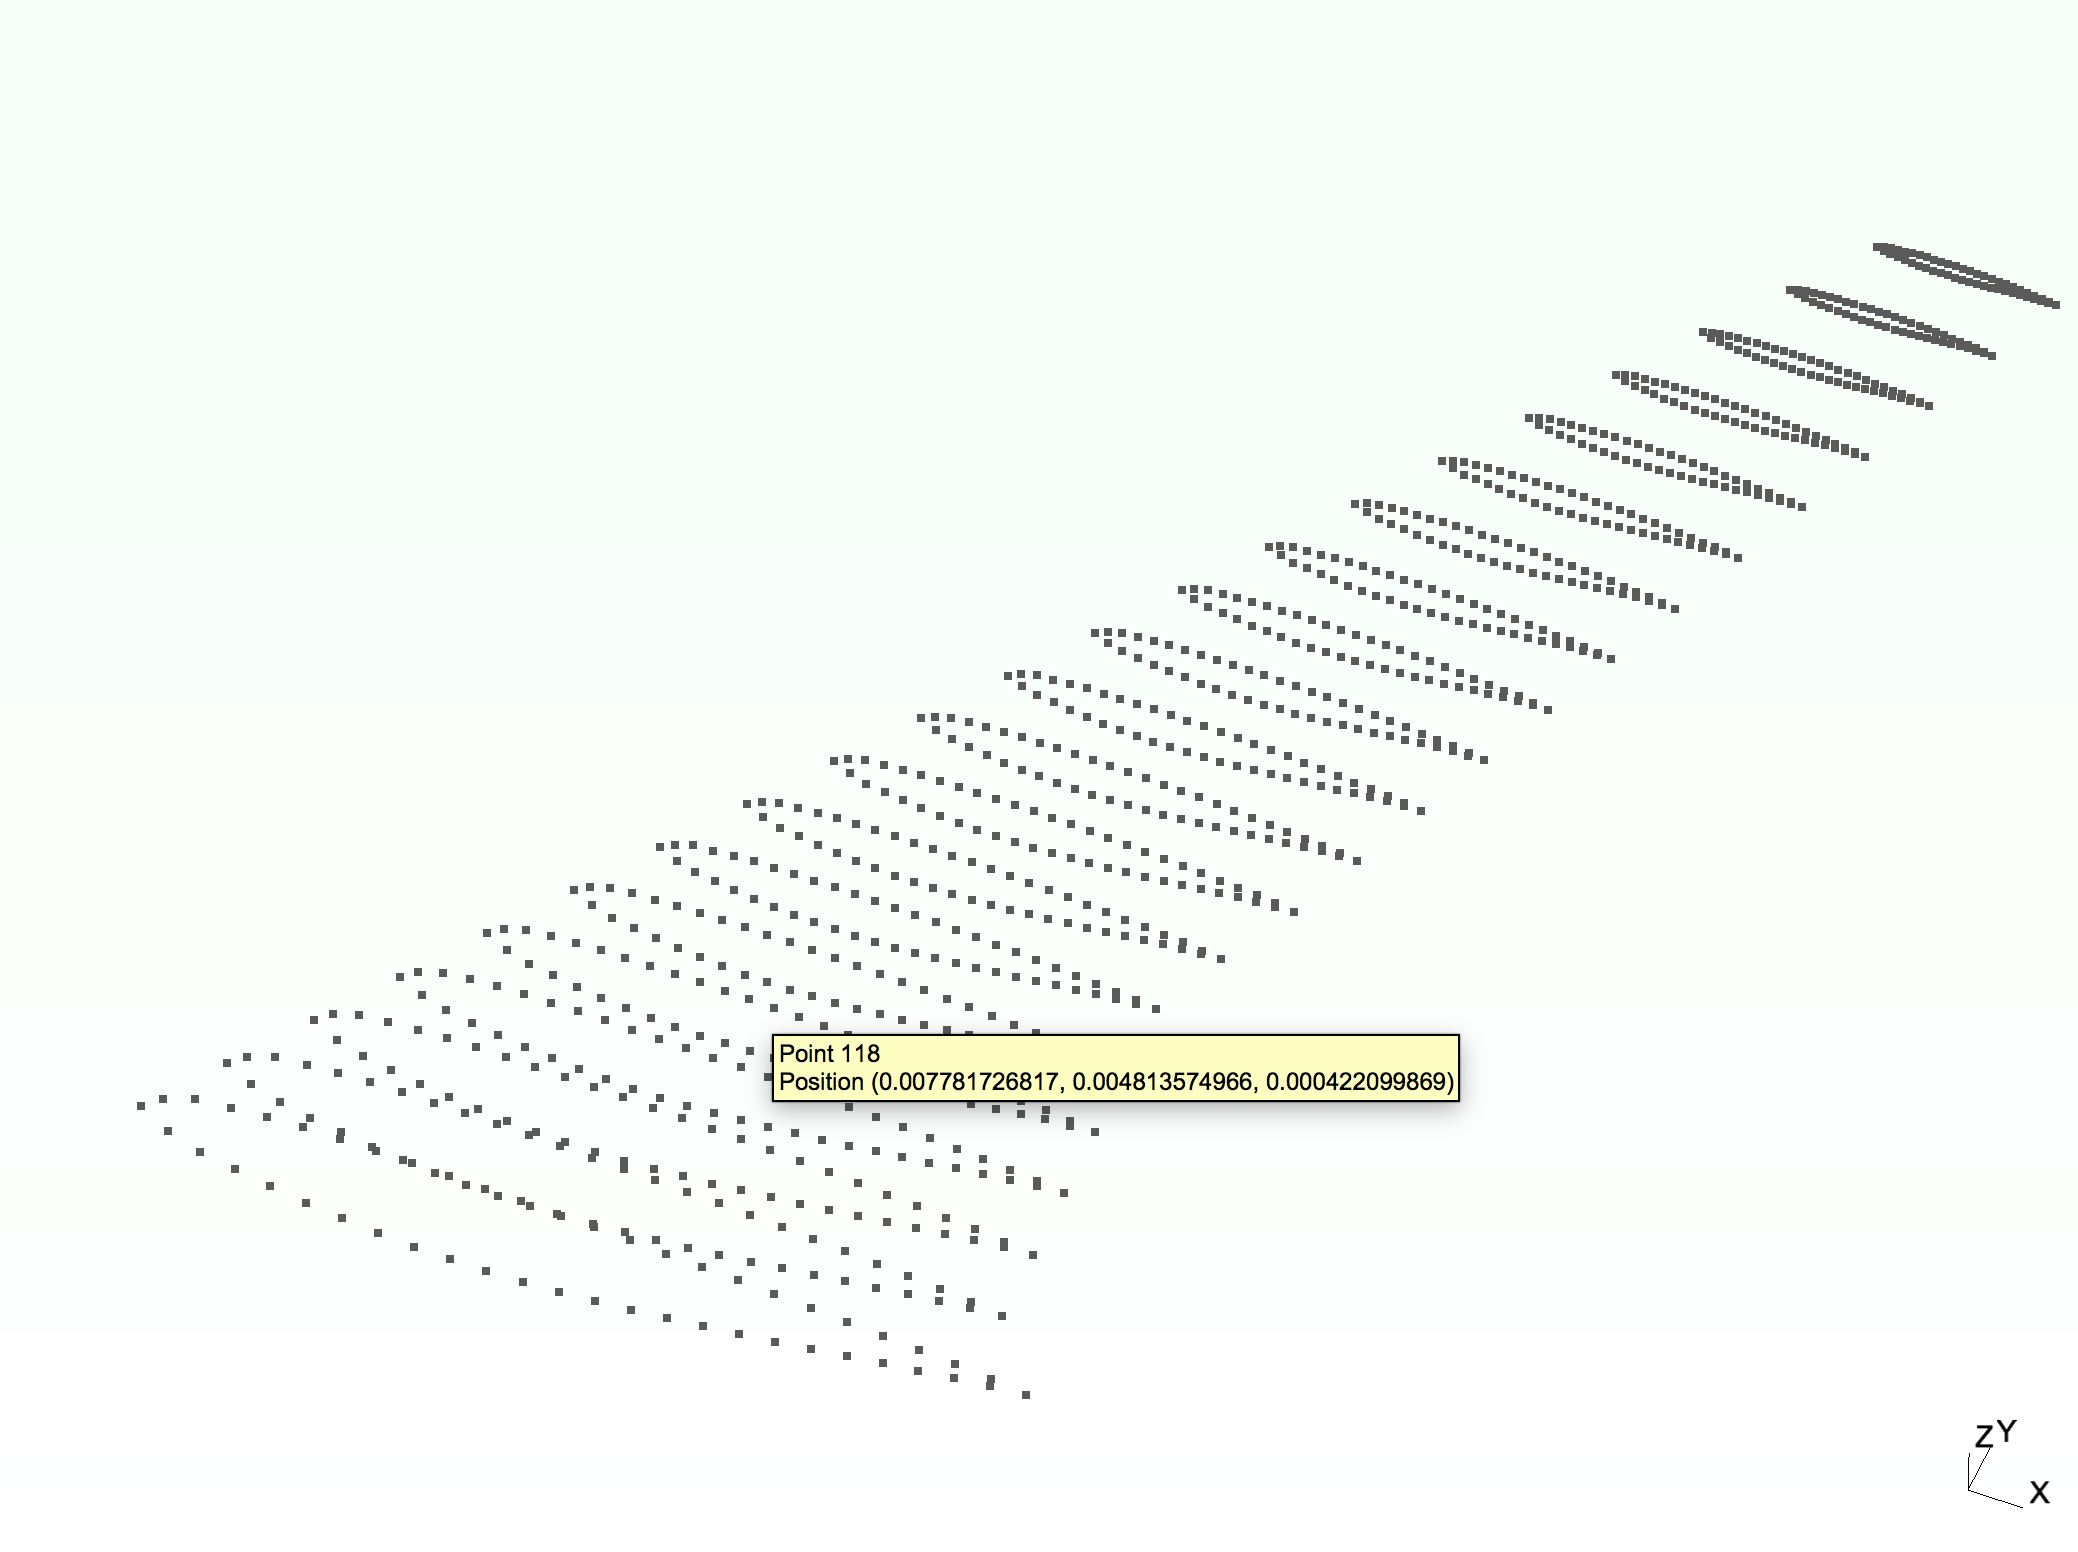
\includegraphics[width = 1\textwidth]{./Immagini/2_2.png}
	\caption{Example of .igs file created from the geometry component}
	\label{fig:2_2}
\end{figure}
\subsection{Raidial Basis Functions}
The second component is the radial basis functions, this component creates the interpolation matrix to couple the aerodynamic and structure component, in fact in the general case these grids are not coincident.The interpolation matrix is created using a fluide-structure interpolation and mesh motion scheme based on the use of radial basis functions (RBF), as the method presented in the work of Rendall and Allen \cite{all}. This displacement and load transfer techniqueis conservative in terms of total load and moment, as shown by Jakobsson and Amoignon. \cite{jac} One of the advantages of this type of interpolations is that no mesh connectivity is required between the two disciplines. This is particularly suitable for the cases where the aerodynamic and structural models do not represent the same geometries. Usually, the aerodynamic grid is based on the outer mold line, even though there may be cases where it is based on the mean camber surface only (e.g., the vortex lattice methods).\cite{joan}\\Once the interpolation matrix \textbf{H} have been created, since the dimensions of the problem will not change until the process, it will hold and it will be used each time the aerodynamic component and the structure component run in order to transfer respectively the aerodynamic forces from the CFD mesh to the FEM mesh and the nodal displacement from the FEM mesh to the CFD mesh.\\
\begin{figure}[H]
	\centering
	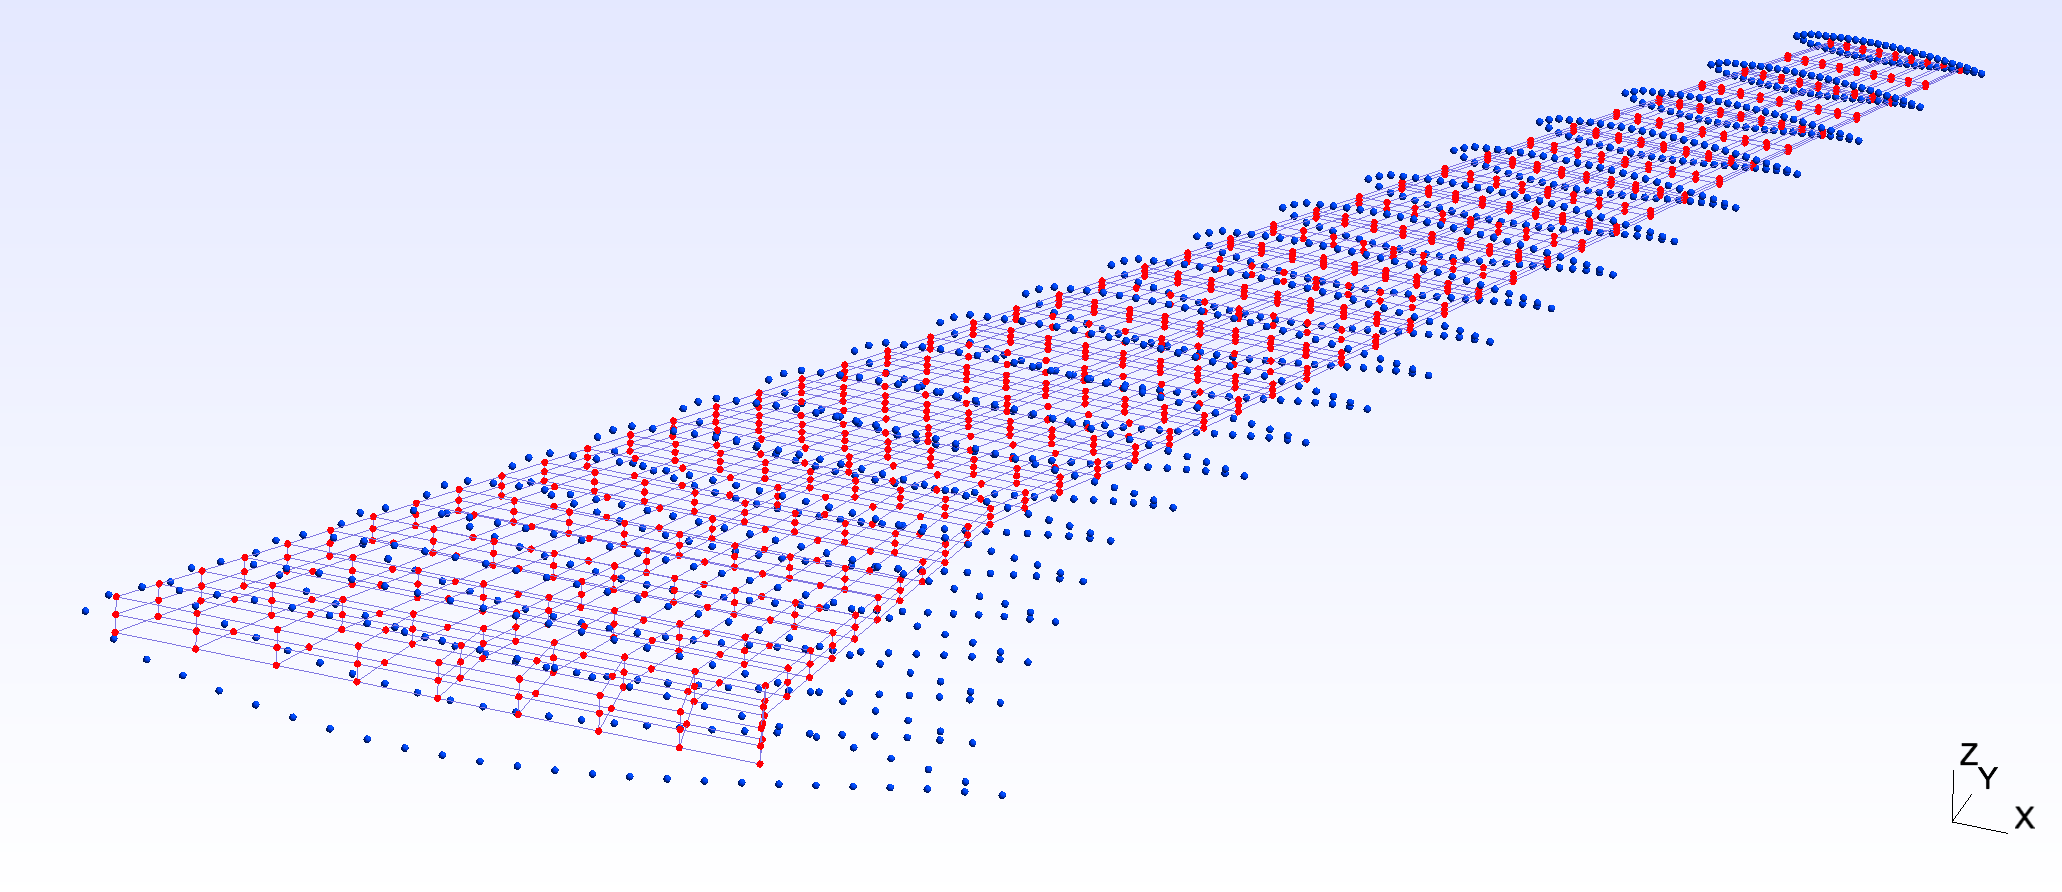
\includegraphics[width = 1\textwidth]{./Immagini/2_3.png}
	\caption{Example of structural mesh (red) and aerodynamic mesh (blue)}
	\label{fig:2_3}
\end{figure}
The input of this component are the outputs of the geometry component, in particular the vector containing the nodes of the CFD mesh $ X_a $ and the vector containing the nodes of the FEM mesh $ X_s $. Instead the output will be the interpolation matrix $ H $. \\This matrix is able to transform the displacements of the structural nodes into displacements of aerodynamic nodes using the formula :
\begin{equation*}
u_a = H \cdot u_s
\end{equation*}
Furthermore, the transpose of this matrix is used to convert the forces of the aerodynamic nodes to the forces of the structural ones with the corresponding formula:
\begin{equation*}
f_s=H^T \cdot f_a
\end{equation*}
\subsection{Aerodynamics}
The aerodynamics component as first creates the shape of the deformed wing by adding the deformation on the initial jig shape, after creates the input file to run an aerodynamic analysis using the external software Panair, than launch Panair, and extracts the aerodynamic characteristics of the wing and stores it into an appropriated dictionary; for each iteration.\\
Once the jig shape is updated, the component creates an auxiliary file that Panin, the input file compiler for Panair, than run Panin in order to get the input file for Panair in a .wgs format.
The aerodynamics loads are computed by means a potential flow panel code, Panair/A502, wich, from an aerodynamic mesh,the value of angle of attack and the Mach, determines the pressure coefficient $C_p$ at the control points of the panel. In order to use the RBF interpolation we need the aerodynamics load on the grid points, so first we use numerical integration of the $C_p$ over the aerodynamic panels and then evenly distributing the total panel forces among the four panel vertexes. A symmetric flow is assumed throughout this work.\\ At the end of process we have a python dictionary which contains the aerodynamics load for each grid point for that iteration.

\subsection{Structure}
The structure component uses the external software Nastran95 to perform the static, and when is request the modal and/or dynamic, analysis of the wing. As first the component takes as input a nastran template file, where is declared the BEGIN BULK section, a sample for each nastran cards used(GRID for nodes, QUAD for shell elements, FORCE1 for the nodal forces, MAT1 for material proprieties,BAR for rod elements \cite{msc}), the mechanical proprieties, the section proprieties, the dictionary containing the coordinates of the structural nodes. Using this parameters the component writes the input files for nastran, where the coordinates of the node from the template file are filled with the dictionary of all structural nodes, and the same for the other nastran card featured in the template file Fig. \ref{fig:2_4}. Until the thickness of the shell elements is assumed as design variables also the thickness vector modified from the optimizer is included in the input variables. Whenever the dynamic analysis is requested it's essential define also the data required for the analysis.\\
When the input file is ready the component launch the nastran software.\\
As for the static structural analysis to compute the displacements of the wing and the stresses of the elements a linear finite element model have been used. The equation that must be solved for the finite element analysis is :
\begin{equation*}
Ku_s=f_s
\end{equation*}
which is linear with respect to the structural displacement, and the stiffness matric $K$ depends only of the material properties and of the underformed geometry, contained in the jig shape. Nastran uses an $LU$ decomposition of the stiffness matrix $K$ to solve the linear system. So seen as structured the problem the $LU$ decomposition of $K$ doesn't change until the optimization process, than it will be stored, and using a $DMAP$ alteration of the FORTRAN code, it will used at the beginning of each MDA loop, to award a computational cost reduction.\\
After the analysis is finished the component takes from the output file (.out for displacement, .pnh for stresses, modal shape, frequencies,$V-g$ and $f-g$ diagrams) the value of the required variables and stores it into an dedicated python dictionary. Nastran can be used also to determinate the mass of the wing, that is an important information, especially when mass is used as objective function. As we will see more detailed in the next chapter, this component can be modified also to extract the mass and inertia properties of a section of the wing, using the nastran weight generator instrument and a unitary load ad nodal forces.
\begin{figure}[H]
	\centering
	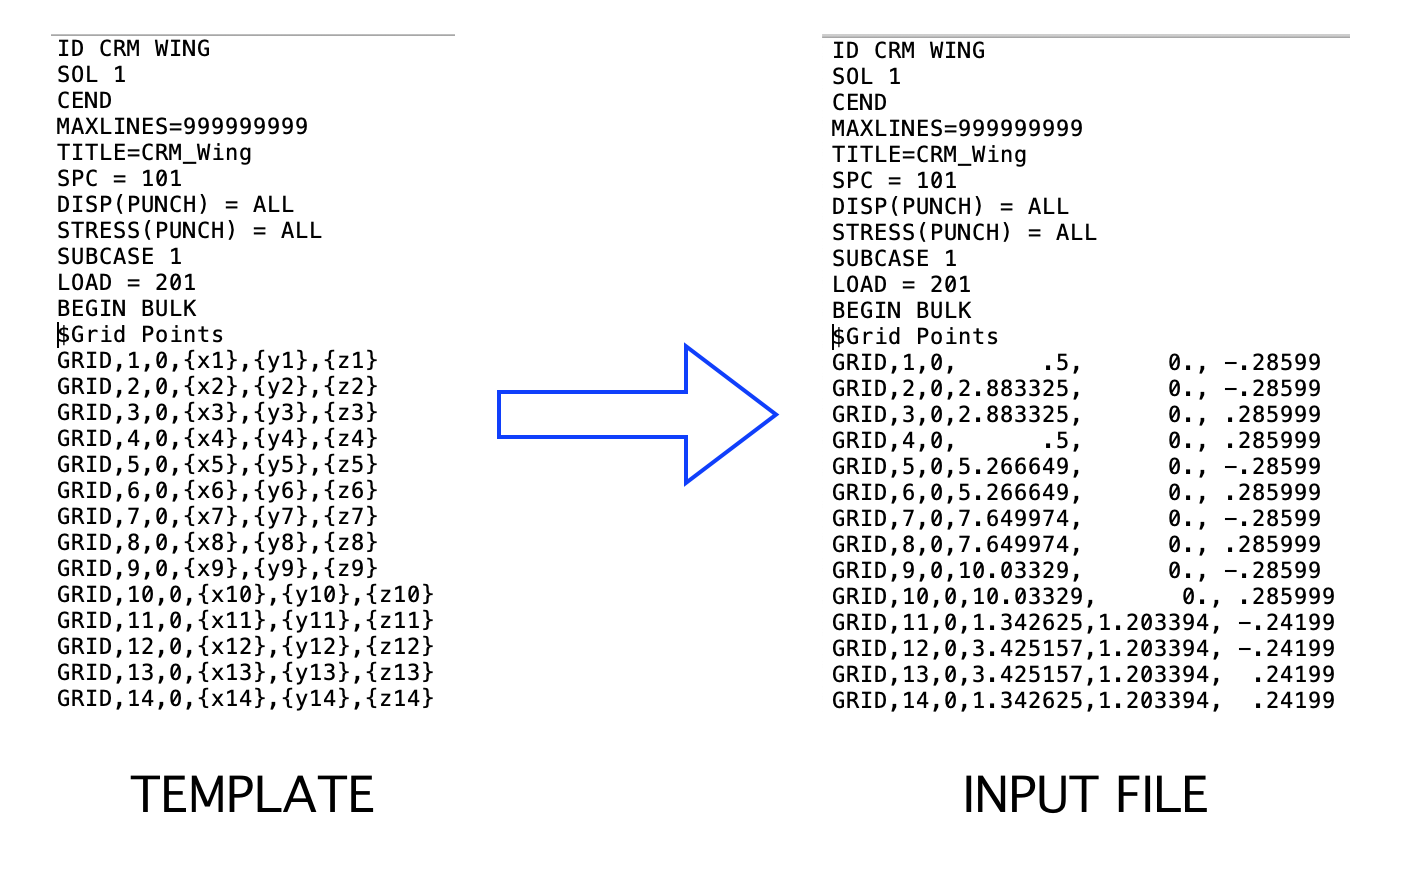
\includegraphics[width = 0.8\textwidth]{./Immagini/2_4.png}
	\caption{Example of nastran template file and input file generated from it}
	\label{fig:2_4}
\end{figure}
\subsection{Load and Displacements Transfer}
In the MDA loop as we said there is coupling between aerodynamic mesh point displacements $u_a$, structural node displacement $u_s$, aerodynamic forces referred on the structural nodes $f_s$ and aerodynamic forces referred on the aerodynamic mesh points.\\
If the aerodynamic mesh is different from the structural mesh it's necessary to interpolate the structural displacement into the aerodynamic mesh points. The displacement interpolation scheme  is based on the work by Rendall and Allen. \cite{all} In that method, each component of the displacement vector \textbf{u} is interpolated as follows (Eq. 2.1 is written for the x component, but the same holds for y and z):
\begin{equation}
u_x=\sum_{i=1}^{N_s}\alpha_i^x\Phi\left(\vert\vert \mathbf{x}-\mathbf{x_i}\vert \vert\right)+\gamma_0^x+\gamma_x^x x+\gamma_y^x y + \gamma_z^x z 
\end{equation}
where $\Phi(r)$ is the form of function adopted. In that case, we choose $\Phi(r)=r^2\ln r$, known as the Thin Plate Spline function (TPS).\cite{joan} According to Lombardi et al. \cite{lomb} who performed a comparison between several available functions, the use of TPS functions is the best and safest option in terms of accuracy of the interpolation. The terms $\alpha_i^x$ are the coefficients of the radial basis functions. Each structural node is the center of an $RBF (\mathbf{x_i})$ and the $\gamma$ terms are the coefficients of the linear polynomial part. By imposing the interpolating condition on these coefficients (the interpolation function evaluated at the structural nodes must be equal to their known displacements) and by evaluating this same function on the aerodynamic grid points, the transformation matrix between the displacements of the structural and aerodynamic points can be expressed as: 
\begin{equation}
u_a=H u_s
\end{equation}
where H is a matrix which depends only on the coordinates of the structural and aerodynamic grid points and the type of RBF chosen.\\
As detailed by Rendall and Allen,\cite{all} and by virtue of the principle of virtual work to ensure the conservation of energy, we can determine the transformation matrix between the aerodynamic forces on the aerodynamic $f_a$ and structural $f_s$ points. The virtual work can be written as:
\begin{equation}
	\delta W = \delta u_s^T \cdot f_s = \delta u_a^T \cdot f_a
\end{equation}
where $\delta u_s$ and $\delta u_a$ are the virtual displacements of the structural and aerodynamic grids respectively. Through the displacement interpolation matrix $H$, we can express the virtual displacements of the aerodynamic grid:
\begin{equation}
\delta u_a=H\delta u_s
\end{equation}
as function of $\delta u_s$. By substituting equation 2.4 into equation 2.3 we get that:
\begin{equation}
	f_s=H^T f_a
\end{equation}
In the case where gradient-based optimization techniques are used for optimization problems that use the aerostructural coupling presented herein, it can be useful to compute the partial derivatives of the coordinates of the deformed aerodynamic mesh $X_a$ with respect to the structural displacements $u_S$, as well as the partial derivatives of the aerodynamic forces on the structural nodes $f_s$ with respect to the forces on the aerodynamic grid points $f_a$.\cite{joan}\\
The deformed aerodynamic mesh is obtained by adding the interpolated displacements (given by equation 2.3) to the jig shape aerodynamic mesh:
\begin{equation}
	X_a=X_a^0+u_a=X_0+Hu_s
\end{equation}
\section{Driver}
In this section is explained how the driver of the problem, the optimization and the aeroelastic coupling driver, is structured. The entirely code is based on the openMDAO structure, so we use  the integrated optimization driver for the optimization loop, and also the integrated equation solver for the aeroelastic coupling loop. Let's see in details how each driver works.
\subsection{Global Optimizer}
The global optimizer controls all the process, it will change the design variables in order to minimize the objective function, each time the design variables change it will launch the mda loop until convergence to determinate the correct aerodynamics loads and structural displacement, and consequently the right stresses, after that it will check if the constraint is respected and the effect of the changes on the objective function, than it will repeat this process until convergence. \\
To define the optimization driver first thing is to choose the optimizer and set the optimizer option, after need to define the objective function, the constraint and the design variables.
\subsubsection{Optimizer}
The optimizer chosen for this problem are two:
\begin{itemize}
	\item \textbf{COBYLA}: a gradient free optimizer
	\item \textbf{SLSQP}: a gradient based optimizer ( in this case gradient will be calculated using finite differences method)
\end{itemize}
In the examples chapter optimization using both method on the same model have done, to see the differences between the two optimization method.
\subsubsection{Design Variables}
In this code several design variables were implemented:
\renewcommand{\labelitemi}{--}
\begin{itemize}
\item The angle of attack $\alpha$
\item The twist angle $\theta$
\item The mid spar position
\item The scale factor
\item The area of stringer
\item The sweep angle $\Lambda$
\item The cord factor
\item The thicknesses of the different section of the wing inputted as an array *
\end{itemize}
* The structural design variables consist of the thicknesses of the structural finite elements. The topology of structure remains unchanged. In the FEM model we divided the QUAD elements in groups, all the elements of the same group has the same thickness. How you can see in Fig. \ref{fig:2_5} there are different group for the upper surface and for the longerons, so we collect all the information about the thickness in an array. During the optimization process the thicknesses array can be set as design variable.
\begin{figure}[H]
	\centering
	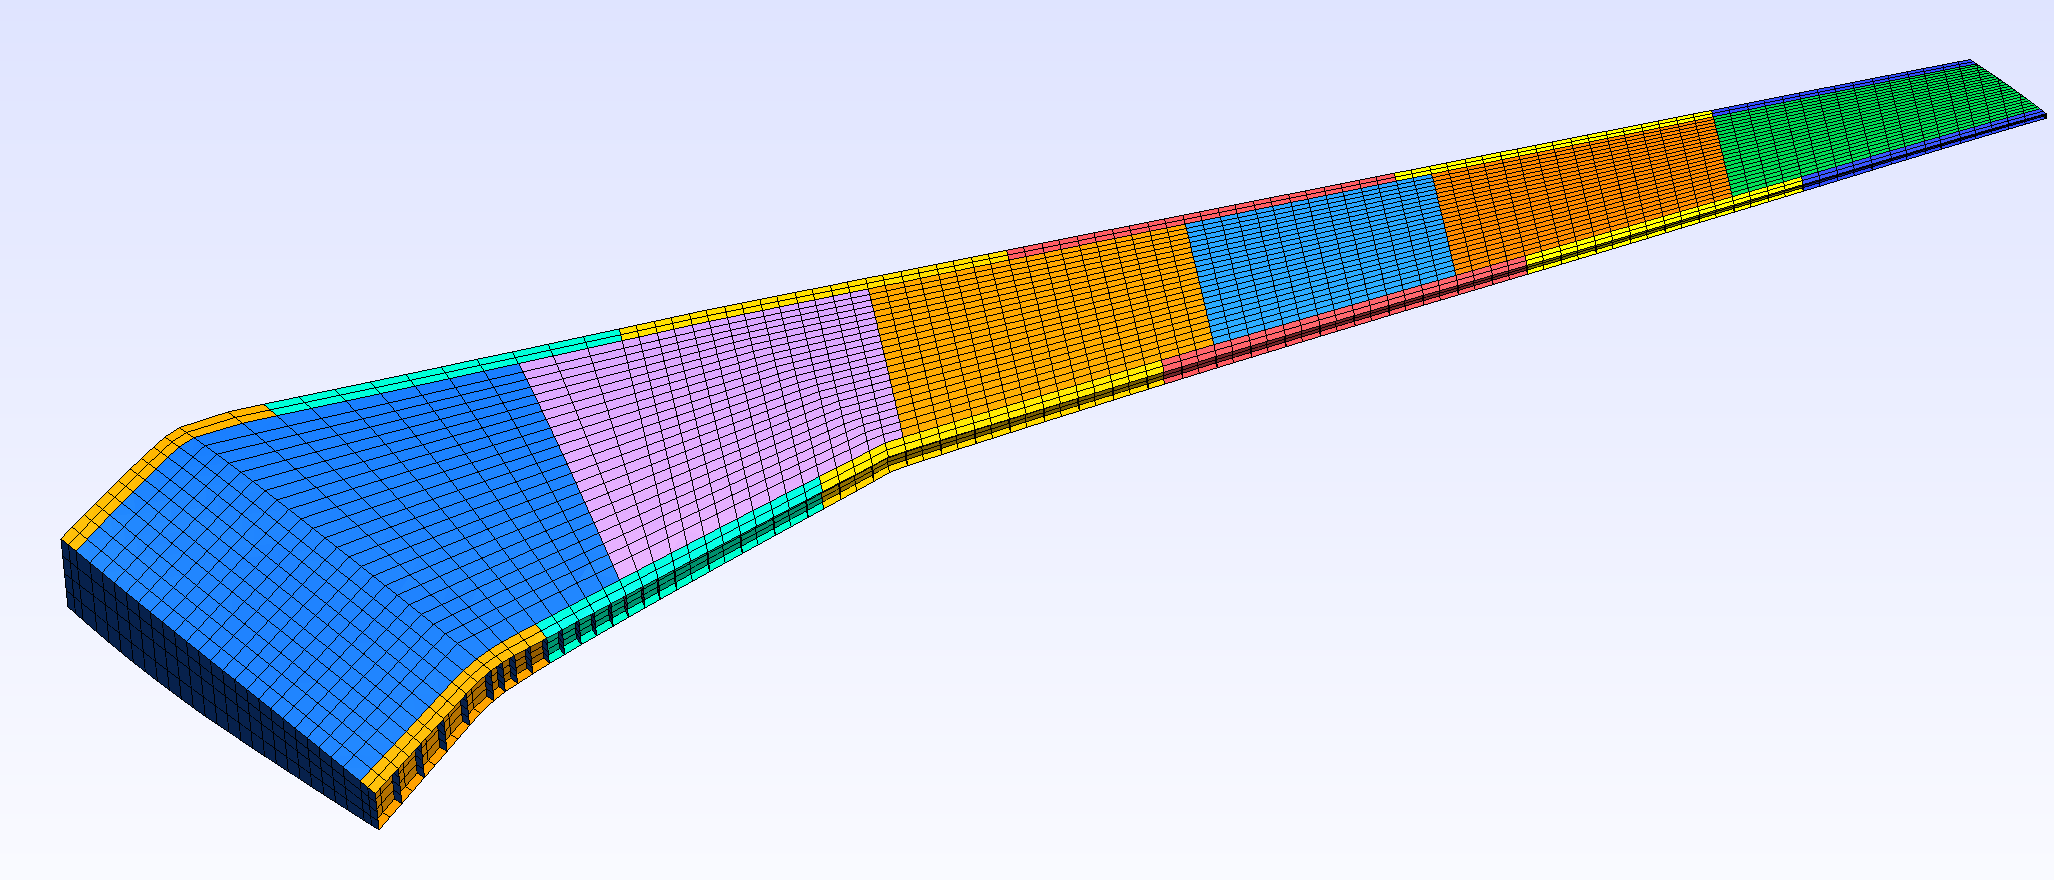
\includegraphics[width = 1\textwidth]{./Immagini/2_5.png}
	\caption{Different thickness sections in the CRM FEM model}
	\label{fig:2_5}
\end{figure}
For each design variable it's possible to set the limits and the initial value. It's possible also to choose just one, a group or all the design variables. In fact in the test cases presented in this work, where the relevant aspect is to test the aggregation component just the angle of attack and the thickness vector is selected as design variables, while all the variables related to the geometry are assumed as constant, so once the geometry is defined it will not change until the process.
\subsubsection{Constraint}
As for the constraints that were imposed, there is one constraint concerning the lift, where the lift must be at least equal to the weight of the aircraft during the cruise, we constrain the $C_L$ by periodically adjusting of the angle of attack of the aircraft within the aero-structural solution until the desired lift is obtained; to set a constraint like this it's necessry to define an \textit{Executable Component}, a component of openMDAO where it's possibile to define a function that is updated for each iteration, and after set this function as constraint imposing the lower or the upper limit. \\In this case the constraint will be:
\begin{equation*}
	C_L - \frac{2W}{\rho_aV^2S_w }> 0
\end{equation*}
The stresses is also considered, so in addition to maintaining the $C_L$ there is also a stress constraint that guarantee the stress of material is lower of the yield stress at the various load condition. The stresses is the result of the structural analysis performed with the finite elements method, so it's necessary to check that the stress of each element respect the constraint, to do this it's necessary to create an \textit{Executable Component} for each element, but usually over than thousand od elements is necessary to describe the structure of the wing, and it becomes computationally very costly to treat these constraints separately. To avoid this problem in the next chapter is explained how we implemented the constraint aggregation.\\ In this case the constraint will be:
\begin{equation*}
\sigma_i - \sigma_{yield} < 0 \ \ \ \ for \ \ \ \ i=1,2,...,N_e
\end{equation*}
where $N_e$ it's the number of finite elements.

\subsubsection{Objective Function}
In the typical aircraft optimization problem the objective is to find the good trade-off between aerodynamic drag and structural weight. So for our optimization problem we set as objective function the induced drag coefficient $C_{D_i}$ and the structural mass $W$, or in the general case a function like:
\begin{equation*}
F = \alpha C_{D_i} + \beta W
\end{equation*}
where $\alpha$ and $\beta$ are scalar parameters that is indicative of the relative importance of the variables that we want to minimize.\\
Is important note that openMDAO is able to manage just minimization problem, so to manage maximization problem is necessary to create an objective function equal to the negative of the real objective function.
\subsection{MDA Driver}
To solve the coupling problem between aerodynamics loads and structural displacements it's necessary an internal loop that through an iterative process which update iteration for iteration the value of the variables implicitly linked reach the convergence. That process is tasked to a non linear equation solver, in this case we choose one of the solver included in the openMDAO library, the non linear Gauss Seidel Solver \textit{NLGaussSeidel} with the aitken accelaration \cite{ait}.\\
To do this the MDA driver call the components that we discussed above in order to reach the convergence. In the Fig. \ref{fig:2_6} it's showed the XDSM concerning the MDA loop: 
\begin{figure}[H]
	\centering
	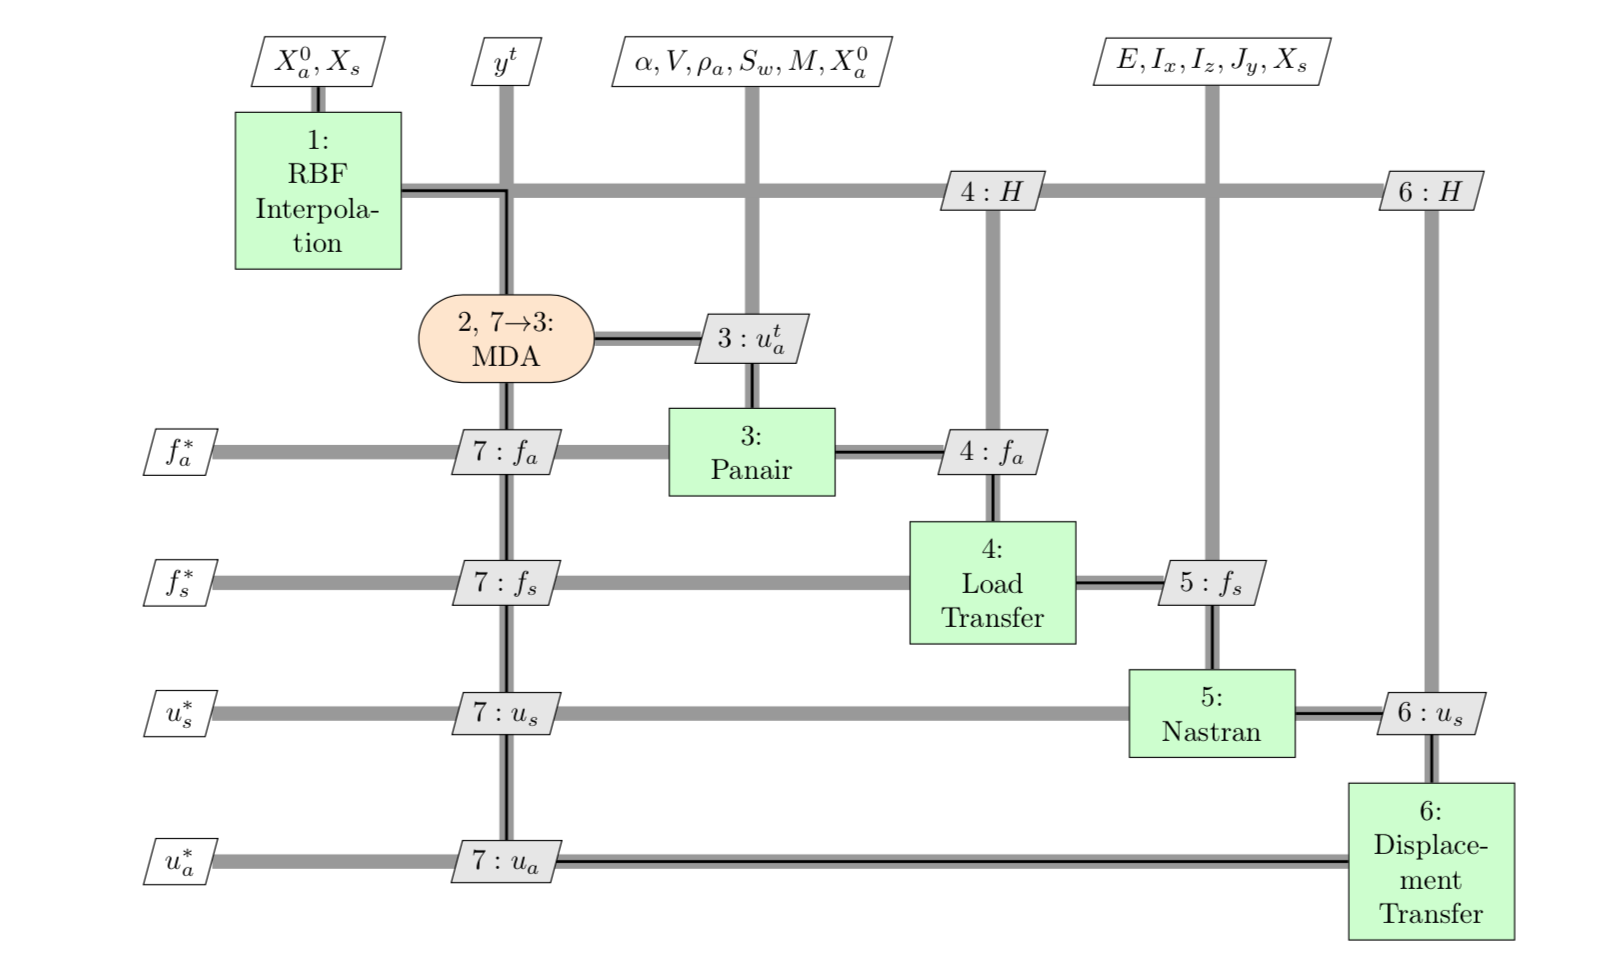
\includegraphics[width = 0.8\textwidth]{./Immagini/2_6.png}
	\caption{XDSM of the MDA Driver}
	\label{fig:2_6}
\end{figure}
The required parameters for each component is the following, fro:
\begin{itemize}
	\item RBF interpolation: the aerodynamic mesh $X_a^0$ and the structural mesh $X_s$;
	\item Aerodynamic analysis: the angle of attack $\alpha$,the flight speed $V$, the density of the air $\rho_a$, the wing surface $S_w$, the Mach $M$;
	\item Structural analysis: the Young module $E$,the barycentric moment of inertia $I_x,\ I_y \ and\  I_z$;
\item Interpolation: the interpolation matrix $H$.
\end{itemize}
	while the coupling variables are $u_a,\ u_s,\ f_a\  and\  f_s$.
The steps to reach the coupling convergence is the following:
\begin{enumerate}
	\item Compute the interpolation matrix $H$.
	\item Initiate the MDA loop.
	\item Compute the aerodynamic forces on the aerodynamic grid points.
	\item Compute the aerodynamic forces on the structural grid points.
	\item Compute the structural displacements.
	\item Compute the aerodynamic grid point displacements
\end{enumerate}
Repeat $3\rightarrow 7$ until convergence.
In Fig. \ref{fig:2_7} it's showed how the vertical displacement of the wingtip nodes change until the process, and how the MDA loop reach the convergence. 
\begin{figure}[H]
	\centering
	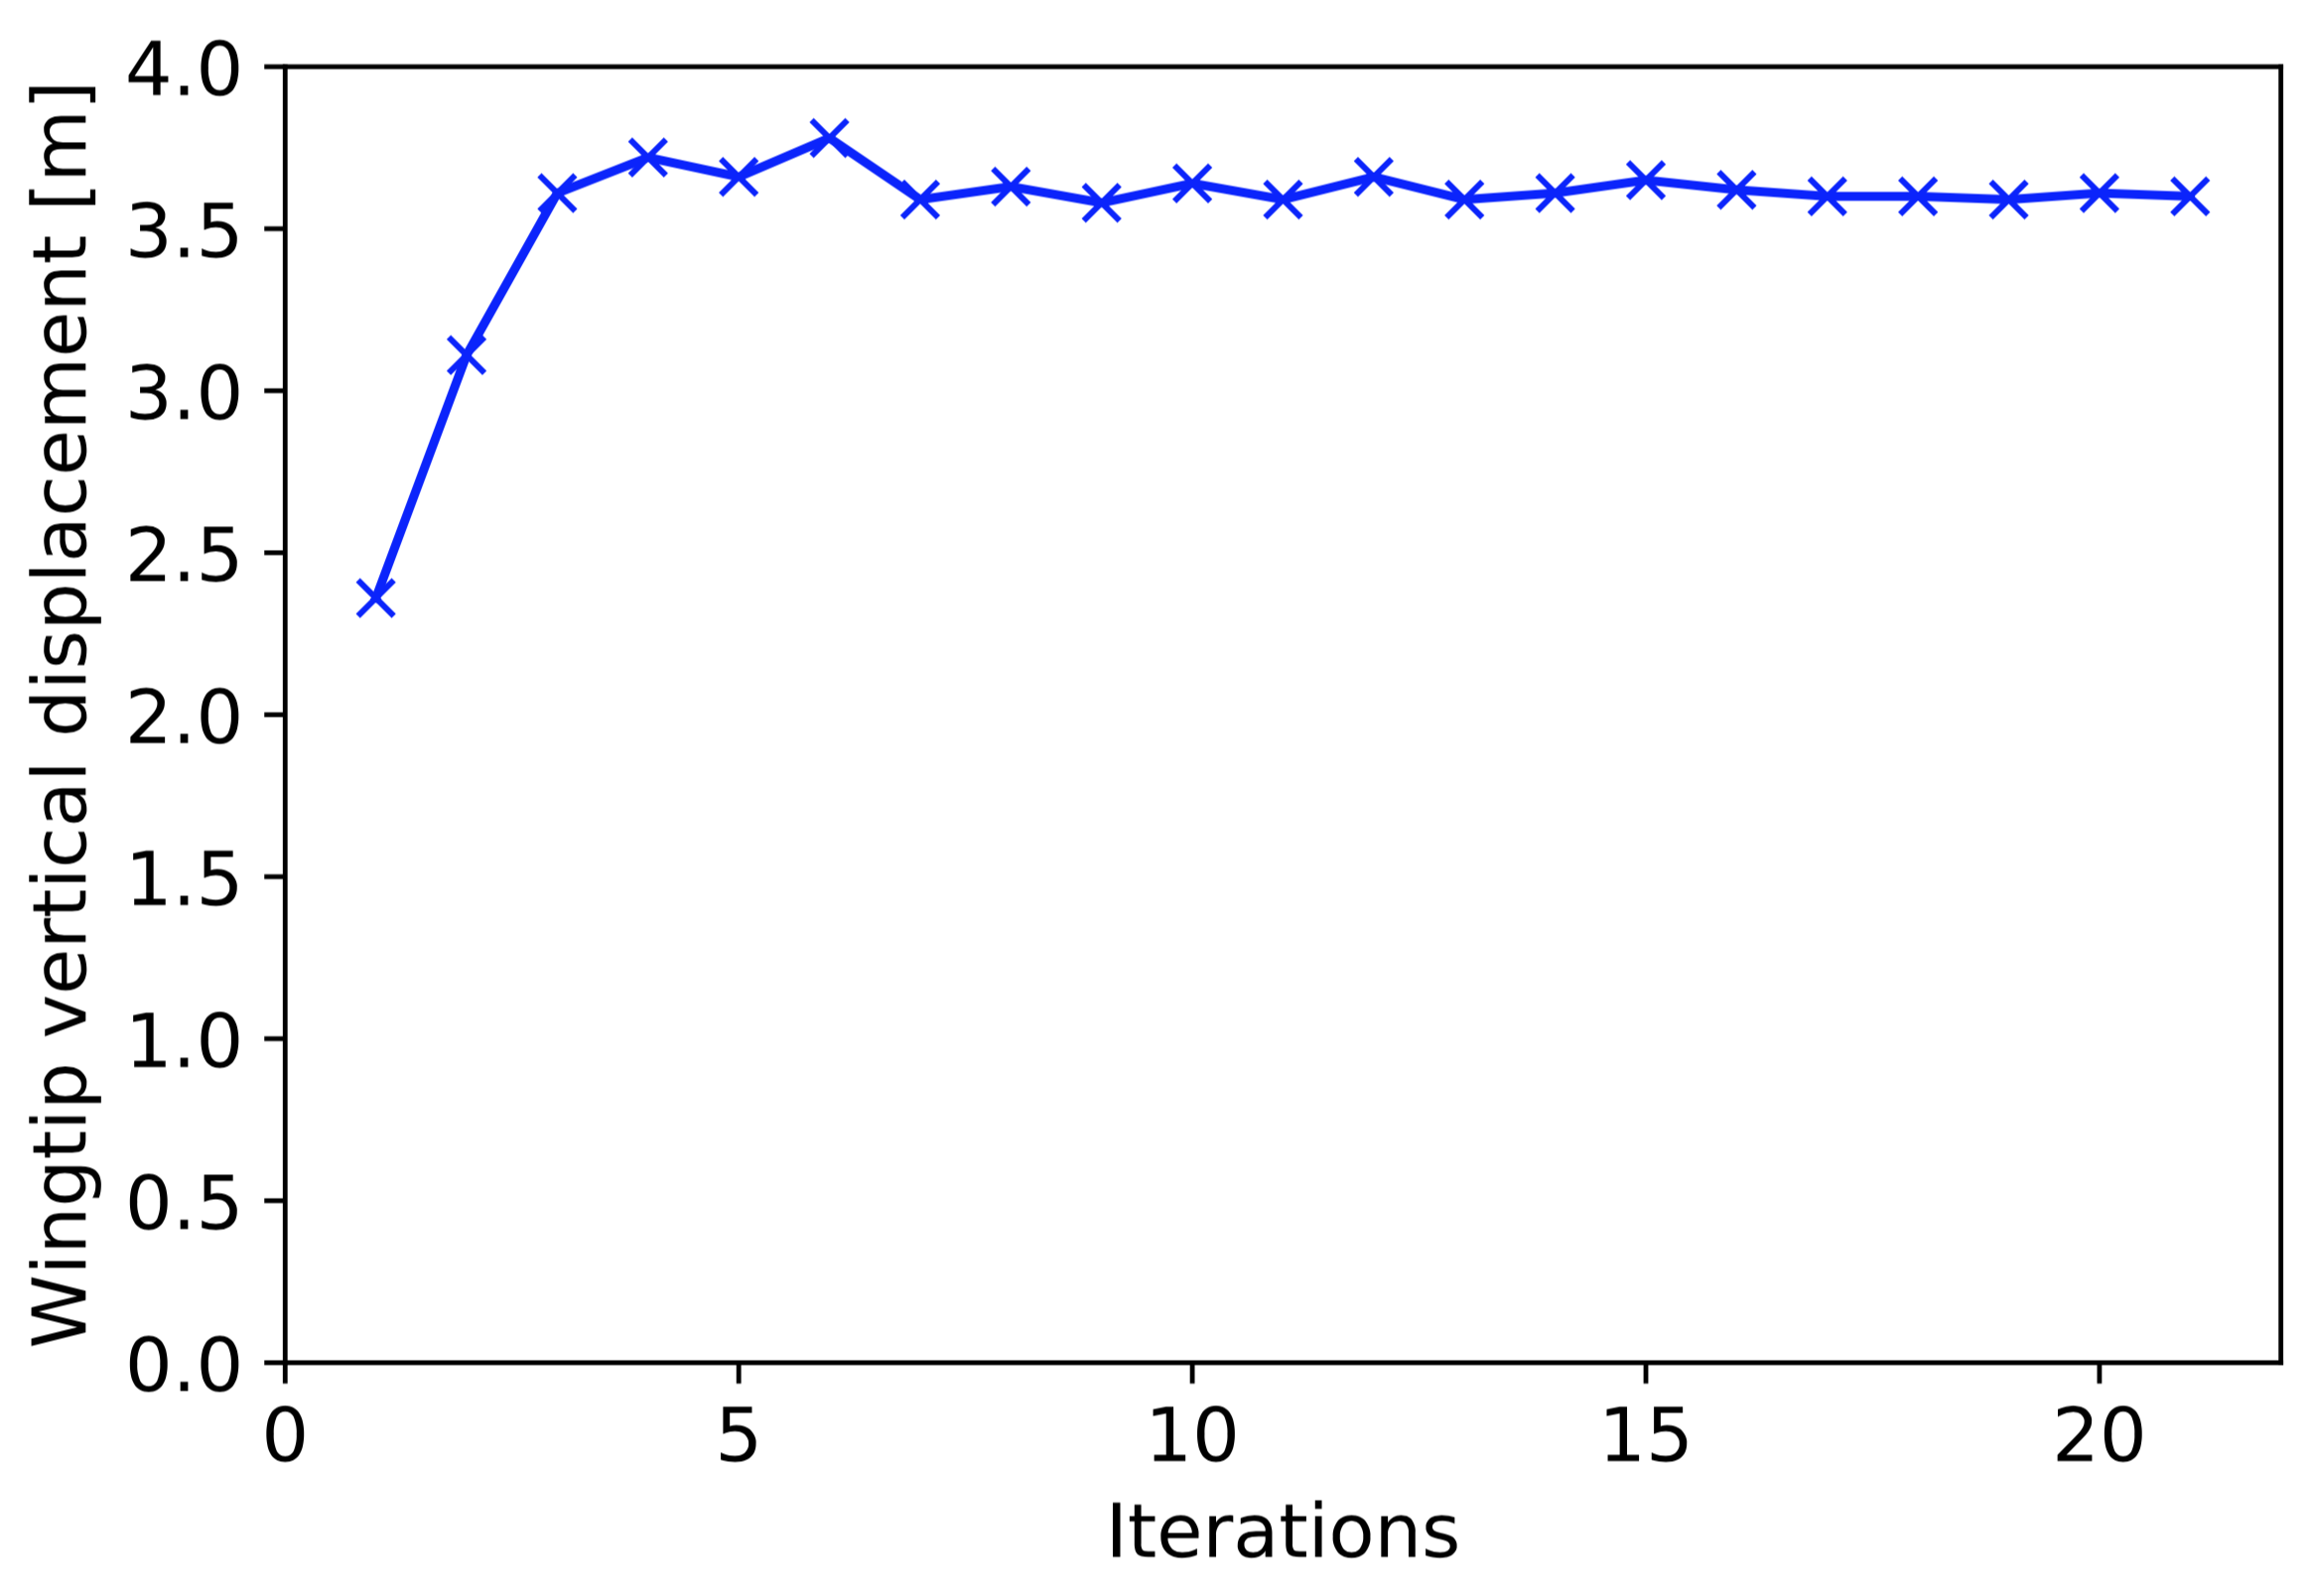
\includegraphics[width = 0.8\textwidth]{./Immagini/2_7.png}
	\caption{Results of the MDA loop refered to the wingtip vertical displacement }
	\label{fig:2_7}
\end{figure}
For each optimization iteration, the MDA loop determinate the displacements and the aerodynamic loading considering the aeroelastic coupling. Normally to reach the convergence needs 6 or 7 iteration, for each iteration one aerodynamic analysis and one static structural analysis is performed, so for high fidelity model, aerodynamic and/or structural, the computational cost can be huge, that's the first reason to introduce a reduce model for the MDA loop, showed in the chapter 4.